\documentclass[12pt,a4paper]{article}

% Paquetes
\usepackage[utf8]{inputenc}
\usepackage[spanish]{babel}
\usepackage{graphicx}
\usepackage{booktabs}
\usepackage{hyperref}
\usepackage{geometry}
\geometry{margin=2.5cm}
\usepackage{float} % para fijar figuras

\title{Informe Técnico: Prueba HiloTools — Pipeline de Datos}
\author{Vhanessa Cardona}
\date{\today}

\begin{document}

\maketitle

\tableofcontents
\newpage

\section{Introducción}

En el contexto actual de las organizaciones modernas, la \textbf{gestión y análisis de datos} 
se ha convertido en un factor crítico para la toma de decisiones estratégicas. 
La disponibilidad de información en múltiples dominios ---ventas, gestión de talento humano 
y control de inventarios--- plantea la necesidad de construir soluciones de \textit{data engineering} 
que permitan integrar, limpiar y transformar datos heterogéneos en un modelo analítico coherente.

La presente prueba técnica tiene como propósito demostrar la capacidad de diseñar un 
\textbf{pipeline de datos end-to-end}, a partir de tres fuentes primarias en formato Excel: 
\texttt{Ventas}, \texttt{RRHH} e \texttt{Inventario}. Estos archivos contienen información 
operacional de una compañía ficticia que requiere ser consolidada en un sistema analítico 
capaz de ofrecer soporte a áreas clave del negocio, tales como el desempeño de empleados, 
la eficiencia del manejo de inventarios y la evolución de las ventas.

Para lograr este objetivo, se plantearon los siguientes pasos principales:

\begin{enumerate}
    \item \textbf{Ingesta y preprocesamiento}: diseño de un módulo robusto que permita consumir 
    los tres ficheros Excel, procesando todas sus hojas de cálculo, manejando valores faltantes, 
    diferencias de formato y decimales con coma. Esta etapa asegura que los datos se encuentren 
    en un formato uniforme y confiable para análisis posteriores.

    \item \textbf{Modelado en estrella}: construcción de un esquema de tipo \textit{star schema}, 
    con una tabla de hechos de ventas y dimensiones que representan clientes, productos, fechas, 
    empleados y almacenes. Este modelo, ampliamente utilizado en entornos de \textit{business intelligence}, 
    garantiza eficiencia en consultas analíticas y claridad en la interpretación de las relaciones entre entidades.

    \item \textbf{Análisis de Componentes Principales (PCA)}: integración de métricas provenientes 
    de ventas, RRHH e inventario en un conjunto de \textit{features} normalizado, sobre el cual se aplica 
    PCA con el fin de identificar patrones latentes y reducir la dimensionalidad del problema. 
    Este análisis facilita descubrir cuáles variables tienen mayor peso en las dinámicas del negocio 
    y cómo se relacionan entre sí.
\end{enumerate}

El resultado final es un \textbf{pipeline reproducible}, empaquetado en un entorno controlado 
(Docker o Conda), documentado en un repositorio GitHub con estructura modular, y acompañado de un informe técnico.  
De esta manera, no solo se busca resolver el caso propuesto, sino también demostrar buenas prácticas 
de ingeniería de datos, claridad en la documentación y capacidad de extraer hallazgos valiosos a partir de información integrada.


\section{Ingesta de datos}

La etapa de ingesta constituye el \textbf{punto de entrada del pipeline}, donde se incorporan y 
estandarizan los datos provenientes de las distintas fuentes primarias. En este caso, 
los tres ficheros provistos en formato Excel (\texttt{sales\_sample.xlsx}, 
\texttt{hr\_sample.xlsx} e \texttt{inventory\_sample.xlsx}) fueron leídos de manera automatizada, 
procesando cada una de sus hojas de cálculo y consolidando la información en un esquema uniforme.

\subsection{Lectura y exploración de ficheros}
Para la lectura inicial se utilizó la librería \texttt{pandas}, que permite manejar archivos Excel 
con múltiples pestañas mediante la función \texttt{pd.ExcelFile}. De esta forma, se logró acceder 
a todas las hojas contenidas en cada fichero sin necesidad de conocer previamente su número o nombre. 
Este enfoque garantiza que el pipeline pueda adaptarse a futuras actualizaciones de las fuentes 
sin modificaciones sustanciales en el código.

Durante esta etapa se efectuó un análisis exploratorio preliminar con el fin de identificar:
\begin{itemize}
    \item Columnas relevantes en cada hoja de cálculo.
    \item Formatos de fecha y presencia de marcas temporales.
    \item Existencia de duplicados o registros inconsistentes.
    \item Uso de comas como separadores decimales.
    \item Posibles valores nulos o incompletos.
\end{itemize}

\subsection{Estandarización de formatos}
Uno de los retos principales en la ingesta fue la heterogeneidad en los formatos de datos. 
Por ejemplo, varias columnas con sufijo \texttt{Date} presentaban registros en formato 
\texttt{YYYY-MM-DD HH:MM:SS}. Estas fueron convertidas de manera uniforme a objetos 
\texttt{datetime} de \texttt{pandas}, lo que permitió posteriores operaciones de filtrado, 
agrupamiento y análisis temporal.

De forma análoga, los valores numéricos que contenían comas como separador decimal fueron 
normalizados al estándar de punto decimal. Esto resultó crucial para evitar errores al momento 
de realizar cálculos de montos, salarios, inventarios y márgenes de ganancia.

\subsection{Manejo de valores nulos y duplicados}
El pipeline se diseñó para ser tolerante a datos incompletos. En lugar de descartar registros, 
se implementaron estrategias de imputación o marcación explícita de valores faltantes, dependiendo 
del contexto de cada columna. Los duplicados, en cambio, fueron eliminados tras validar que no 
aportaban información adicional y que correspondían a errores de carga o repetición.

\subsection{Exportación a formato analítico}
Una vez normalizados, los datos fueron exportados en formato \texttt{parquet}, que ofrece ventajas 
en términos de compresión, eficiencia de lectura/escritura y compatibilidad con entornos analíticos 
modernos. Cada hoja de Excel fue almacenada en un fichero \texttt{.parquet} independiente, ubicado 
en la carpeta \texttt{/data/processed}. Este diseño modular facilita la trazabilidad de los datos 
y permite realizar transformaciones adicionales sin necesidad de procesar de nuevo los archivos brutos.

\subsection{Reproducibilidad}
Finalmente, toda la lógica de ingesta fue encapsulada en scripts dentro de la carpeta 
\texttt{/ingest}, con funciones auxiliares en \texttt{utils\_ingest.py}. Este módulo garantiza que 
la ingesta pueda ejecutarse tanto en un entorno local (\texttt{conda}) como en un contenedor 
\texttt{Docker}, preservando la reproducibilidad y estandarizando el flujo de datos de extremo a extremo.


\section{Modelo en estrella}

El modelo en estrella es una técnica de modelado dimensional utilizada en entornos 
analíticos y de inteligencia de negocios, cuyo objetivo principal es optimizar la 
consulta de grandes volúmenes de datos. En este proyecto se diseñó un esquema en 
estrella a partir de los datos de ventas, recursos humanos e inventarios, 
integrando múltiples dominios en una única vista analítica coherente.

\subsection{Diseño del esquema}
En el centro del modelo se encuentra la \textbf{tabla de hechos de ventas (FactSales)}, 
que consolida las transacciones individuales con métricas cuantitativas tales como:
\begin{itemize}
    \item \texttt{quantity}: número de unidades vendidas.
    \item \texttt{unit\_price}: precio unitario al momento de la venta.
    \item \texttt{discount\_percent}: descuentos aplicados.
    \item \texttt{sales\_amount}: monto total de la transacción.
    \item \texttt{profit\_margin}: margen estimado asociado a la venta.
\end{itemize}

Rodeando la tabla de hechos se definieron las dimensiones que aportan el contexto 
necesario para el análisis multidimensional:
\begin{itemize}
    \item \textbf{DimCustomer}: información de clientes (ID, nombre, segmento).
    \item \textbf{DimProduct}: catálogo de productos y categorías.
    \item \textbf{DimStore}: localización física de las tiendas.
    \item \textbf{DimDate}: calendario estandarizado para análisis temporal.
    \item \textbf{DimEmployee}: desempeño y características de empleados.
    \item \textbf{DimDepartment}: estructura organizacional vinculada a RRHH.
    \item \textbf{DimWarehouse}: almacenes donde se controla el inventario.
    \item \textbf{DimCategory}: clasificación de productos según inventarios.
\end{itemize}

\subsection{Esquema resultante}
La Figura \ref{fig:star_schema} muestra el diagrama resultante del modelo en 
estrella, donde se observa la tabla de hechos en el centro y las dimensiones 
conectadas en torno a ella.

\begin{figure}[H]
    \centering
    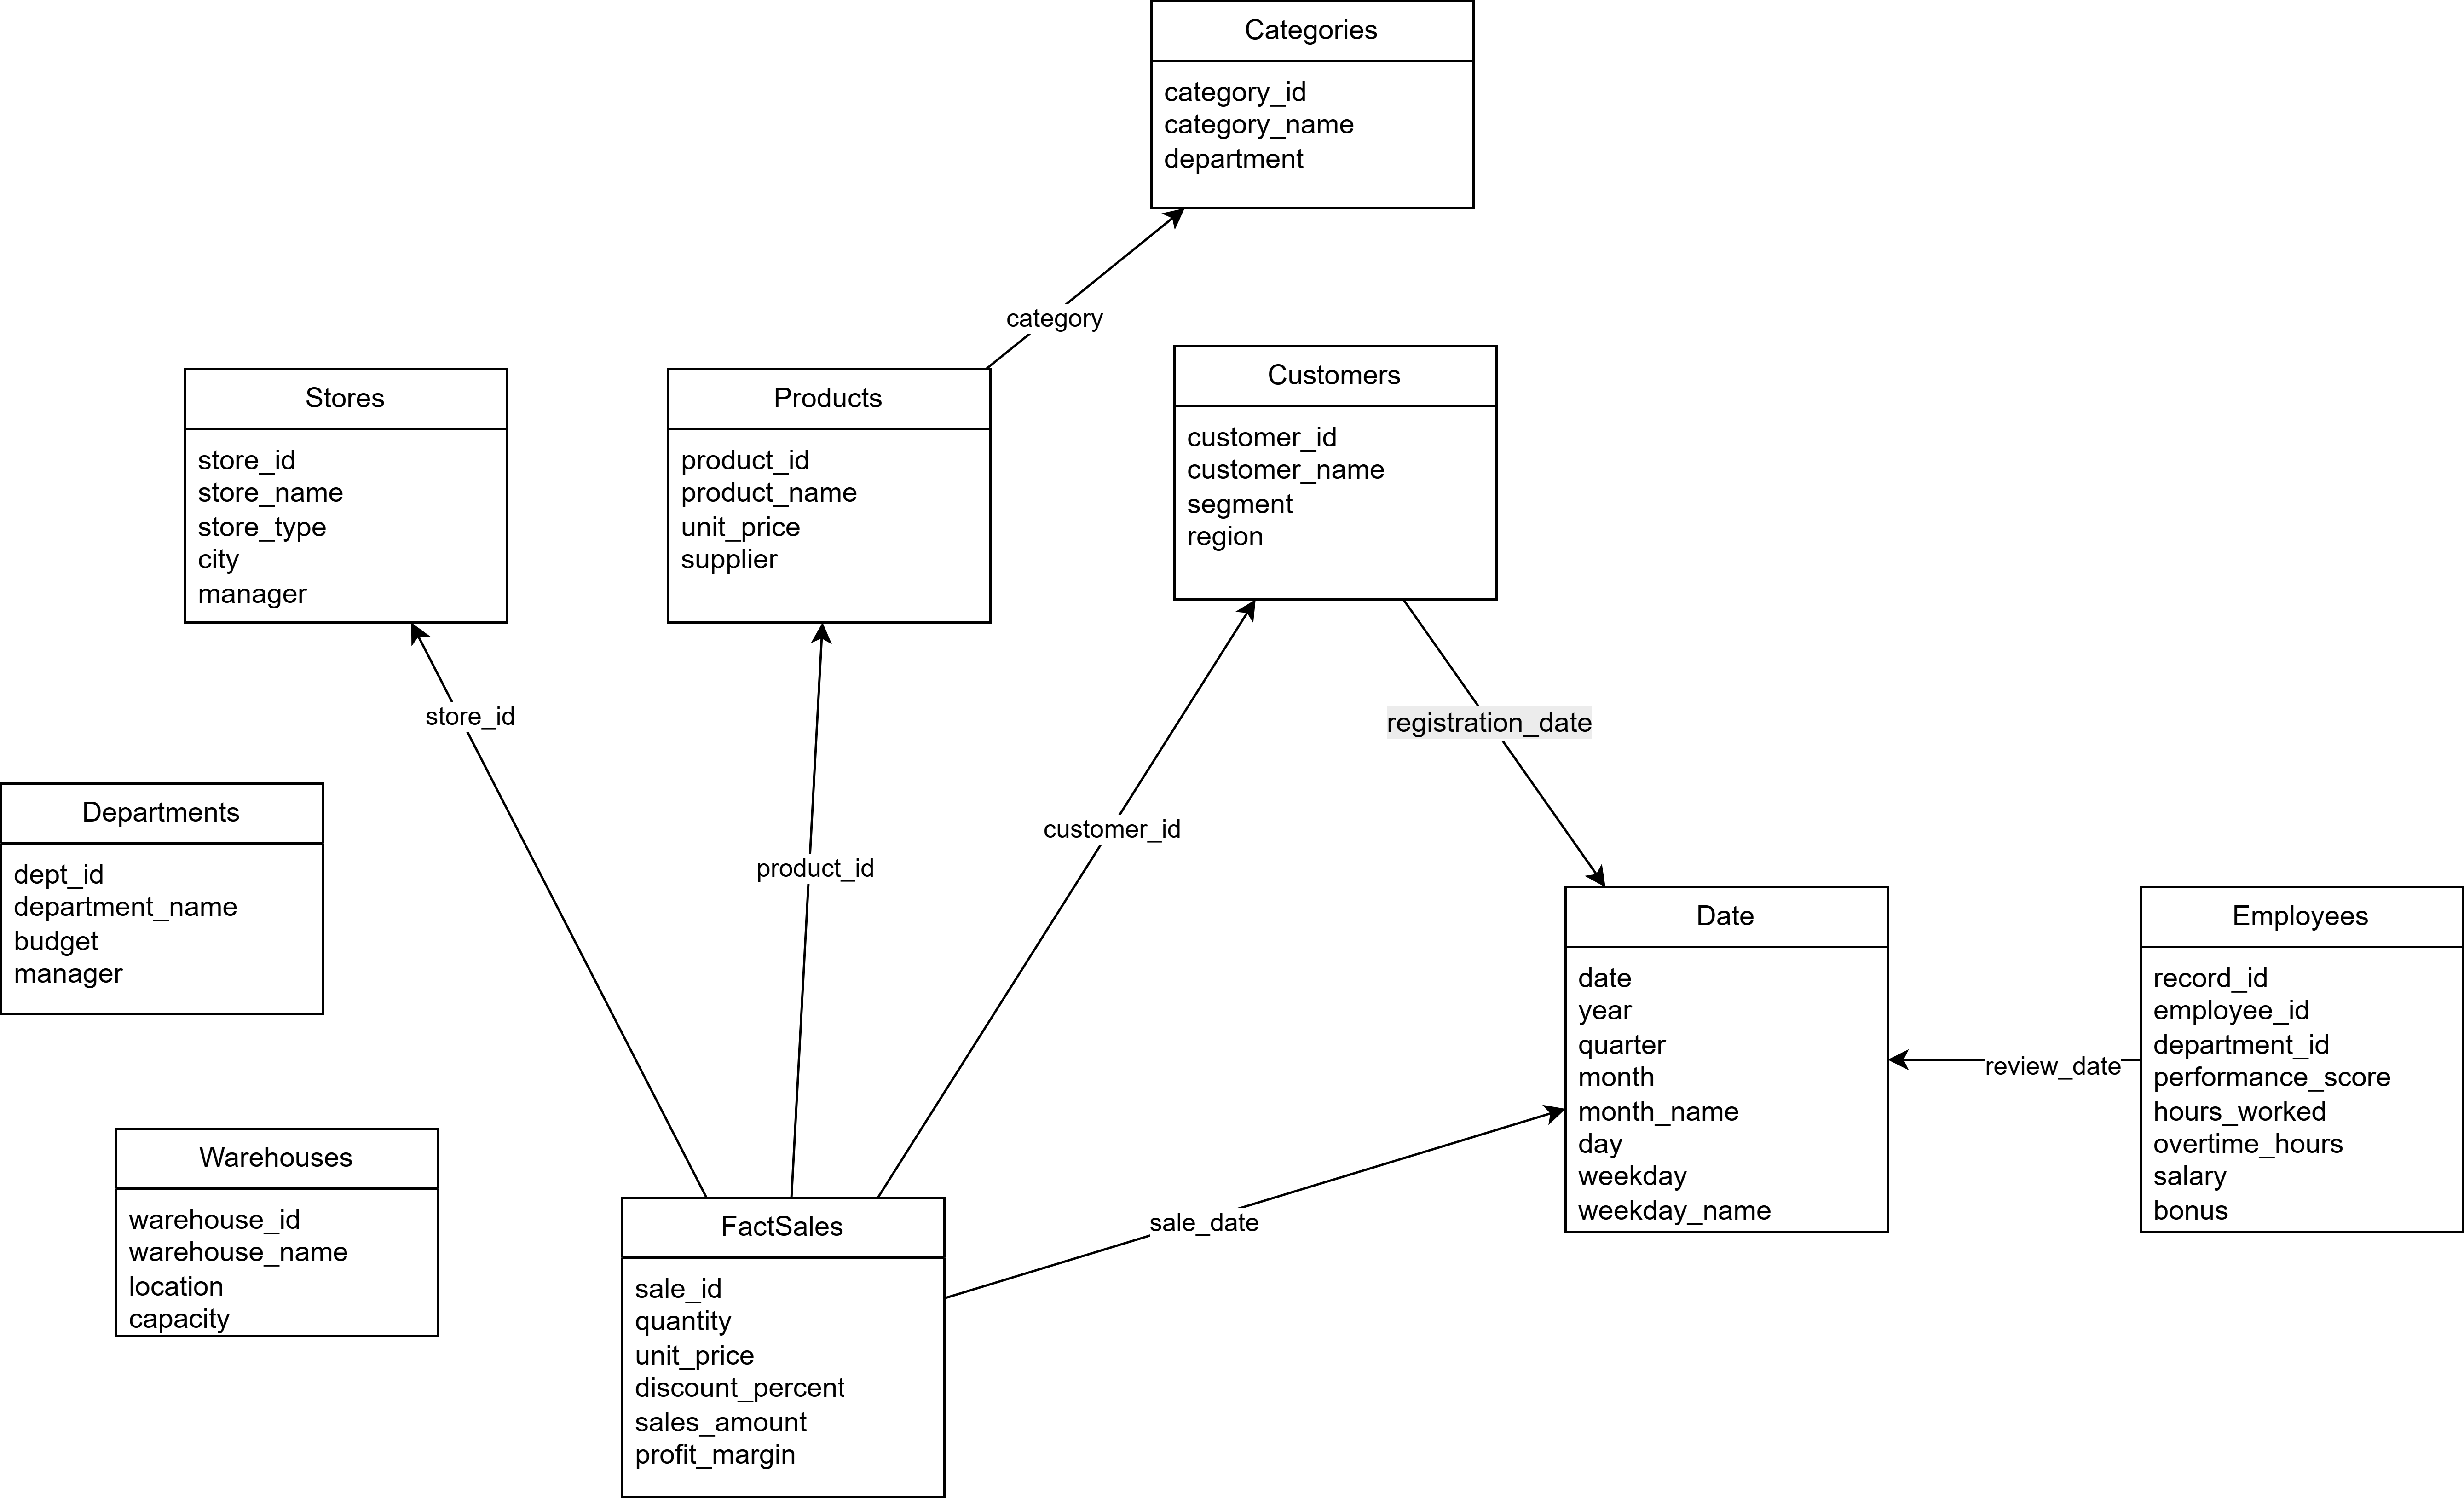
\includegraphics[width=0.9\textwidth]{figures/star_schema.png}
    \caption{Esquema en estrella integrado a partir de ventas, RRHH e inventarios.}
    \label{fig:star_schema}
\end{figure}

\subsection{Ventajas del modelo}
El modelo en estrella ofrece múltiples beneficios:
\begin{itemize}
    \item Simplicidad conceptual: los usuarios pueden comprender fácilmente la 
    relación entre hechos y dimensiones.
    \item Eficiencia en consultas: optimiza el rendimiento de agregaciones y filtros 
    en grandes volúmenes de datos.
    \item Flexibilidad analítica: permite análisis combinados, como identificar el 
    impacto de la rotación de empleados en las ventas o la relación entre niveles de 
    inventario y márgenes de ganancia.
\end{itemize}


\section{Análisis de Componentes Principales (PCA)}

El análisis de componentes principales (PCA, por sus siglas en inglés) es una técnica 
estadística de reducción de dimensionalidad que permite identificar patrones latentes 
en los datos, disminuyendo la redundancia y resaltando las variables que más aportan 
a la variabilidad del sistema. En este proyecto se aplicó PCA para integrar la 
información proveniente de ventas, recursos humanos e inventarios, con el fin de 
detectar relaciones ocultas entre métricas de desempeño, márgenes de rentabilidad y 
gestión de inventarios.

\subsection{Varianza explicada}
Se seleccionaron un conjunto de variables cuantitativas relevantes (ventas, descuentos, 
costos, márgenes, horas trabajadas, entre otras) y se aplicó un PCA con normalización 
previa. El resultado mostró que las \textbf{cinco primeras componentes principales} 
explican cerca del \textbf{80\% de la varianza acumulada}, lo que indica que una 
proporción significativa de la información contenida en los datos puede ser representada 
en un espacio de menor dimensión sin pérdida sustancial de contenido.

\begin{figure}[H]
    \centering
    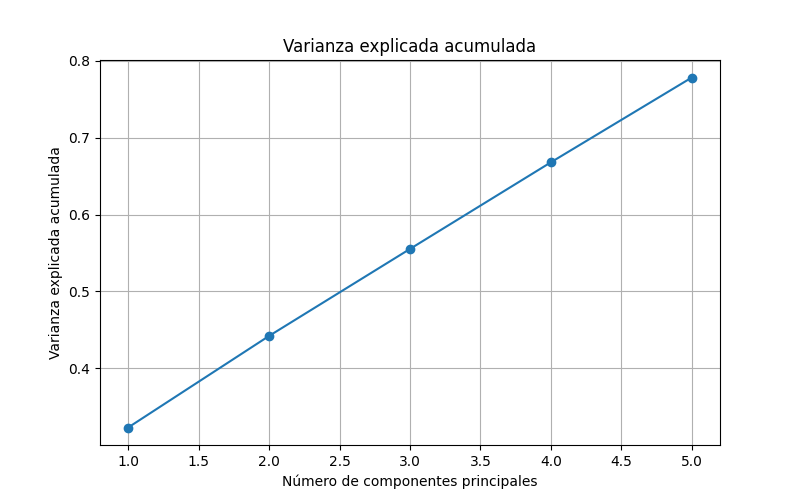
\includegraphics[width=0.7\textwidth]{figures/pca_variance.png}
    \caption{Varianza explicada acumulada por las primeras componentes principales.}
    \label{fig:pca_variance}
\end{figure}

\subsection{Correlaciones por componente}
Para interpretar el significado de cada componente, se analizaron las cargas de 
correlación entre las variables originales y las componentes principales. Los 
hallazgos más relevantes fueron:
\begin{itemize}
    \item \textbf{PC1}: fuerte asociación con las variables \texttt{sales\_amount} y 
    \texttt{profit\_margin}, lo que sugiere que esta componente captura principalmente 
    la dinámica de rentabilidad y volumen de ventas.
    \item \textbf{PC3}: alta correlación con \texttt{discount\_percent}, lo cual 
    refleja la influencia de las políticas de descuentos en el comportamiento de las 
    ventas.
    \item \textbf{PC4}: marcada relación con \texttt{product\_id}, lo que indica que 
    esta componente está asociada a características particulares de los productos 
    (segmentación o tipología).
\end{itemize}

\begin{figure}[H]
    \centering
    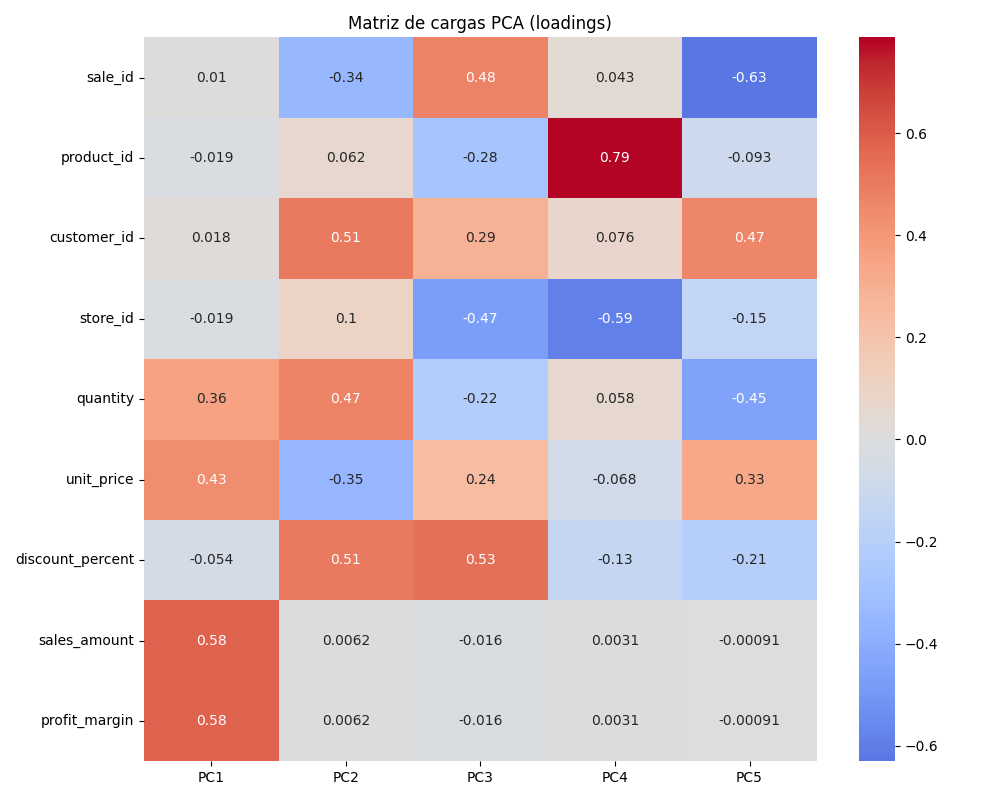
\includegraphics[width=0.8\textwidth]{figures/pca_loadings_heatmap.png}
    \caption{Mapa de calor de correlación entre variables originales y componentes principales.}
    \label{fig:pca_heatmap}
\end{figure}

\subsection{Interpretación}
El análisis PCA permitió resumir la complejidad del dataset en un número reducido de 
dimensiones con interpretación económica y de negocio:
\begin{itemize}
    \item La primera componente representa la \textbf{dimensión de rentabilidad}, 
    explicando gran parte de la varianza.
    \item La tercera y cuarta componentes están más vinculadas a \textbf{estrategias 
    comerciales} (descuentos) y a \textbf{atributos de productos}.
    \item En conjunto, las cinco primeras componentes ofrecen una base sólida para 
    segmentar clientes, evaluar desempeño de empleados y planificar inventarios en 
    función de patrones latentes.
\end{itemize}


\section{Conclusiones}

El desarrollo de este pipeline de datos permitió demostrar la integración de diversas 
fuentes heterogéneas (ventas, recursos humanos e inventarios) en un modelo analítico 
coherente y reproducible. A partir de la experiencia obtenida, se pueden destacar 
las siguientes conclusiones:

\begin{itemize}
    \item \textbf{Ingesta robusta:} Se diseñó un proceso de ingesta capaz de manejar 
    múltiples hojas de cálculo, formatos inconsistentes, valores nulos y diferencias 
    en el uso de separadores decimales. Esto garantiza una base sólida para futuros 
    procesos de automatización.

    \item \textbf{Modelo estrella integrado:} La construcción del esquema en estrella 
    permitió centralizar la tabla de hechos de ventas (\texttt{FactSales}) y vincularla 
    con dimensiones clave como clientes, productos, empleados, almacenes y fechas. 
    Este diseño facilita tanto la escalabilidad como la generación de reportes analíticos.

    \item \textbf{Análisis PCA:} La aplicación de componentes principales reveló que 
    cinco dimensiones explican cerca del 80\% de la varianza en los datos. Se 
    identificaron patrones relevantes, tales como:
    \begin{itemize}
        \item La \textbf{dimensión de rentabilidad} (PC1), asociada a 
        \texttt{sales\_amount} y \texttt{profit\_margin}.
        \item La \textbf{dimensión comercial} (PC3), fuertemente influenciada por 
        \texttt{discount\_percent}.
        \item La \textbf{dimensión de producto} (PC4), relacionada con 
        \texttt{product\_id}.
    \end{itemize}
    Estos hallazgos ofrecen información valiosa para segmentar estrategias de ventas, 
    optimizar inventarios y evaluar el desempeño organizacional.

    \item \textbf{Buenas prácticas:} El proyecto se estructuró bajo una organización 
    modular de carpetas (/ingest, /model, /analytics, /report), promoviendo la 
    reproducibilidad, escalabilidad y mantenibilidad del código en entornos locales 
    y contenedores (Docker).
\end{itemize}

En síntesis, el pipeline desarrollado no solo responde a los requerimientos de la 
prueba técnica, sino que sienta las bases para una plataforma analítica más amplia, 
capaz de adaptarse a nuevos flujos de datos y de evolucionar hacia aplicaciones de 
inteligencia empresarial y ciencia de datos más avanzadas.


\begin{thebibliography}{9}
\bibitem{pandas} Pandas Documentation, \url{https://pandas.pydata.org/}
\bibitem{sklearn} Scikit-Learn Documentation, \url{https://scikit-learn.org/}
\bibitem{hilotools} Enunciado oficial de la prueba técnica HiloTools.
\end{thebibliography}

\end{document}

